\section{Seasonal cycle of the haze extinction}

In order to provide a detailed explanation of the complex latitudinal variability of the detached haze layer, we present
some of the key images that we have analyzed. Based on our previous work focused on the evolution of the detached haze in the
equatorial region \citep{West2018}, we define four different seasonal phase characteristics of the evolution of the detached haze layer.
Between 2004 and 2008, the DHL was stable in altitude and extinction.
Between 2008 and 2012, it settled, merged and finally disappeared in the main haze.
During the period 2012-2016, the DHL was not observed and only sporadic transitory layers showed up.
After 2016 and up to the end of Cassini mission, the DHL reappeared following a complex pattern.
The complete survey is performed along a period of time which represents about half a Titan year.
This is valuable because it encompasses the equinoctial transition period of 2009.
For each phase, we display the altitude and latitude distribution of the instantaneous haze extinction retrieved from intensities at the illuminated limb of Titan.
The same color scale is applied to all the panels in order to keep a consistent view on the whole dataset.
Locations where no data are available are left as blank areas on the panels.

\subsection{Period 1: Stable detached haze Layer during the Northern Winter (2004-2008) - $L_s=\ang{300}-\ang{340}$}

At its arrival in the Saturnian system in 2004, Cassini observed a single detached haze layer at 500 km altitude 
(Fig.~\ref{fig:dhl_2004_2008}a) similar to the one observed at 350 km by Voyager 24 years before
\citep{Smith1981}. At that moment, Titan was two years after the winter solstice in the northern hemisphere, at $L_s=\ang{300}$.
With Cassini, we see that, in the southern hemisphere, the haze layer was completely detached from the main haze layer.
The haze extinction was at least one order of magnitude smaller inside the depleted zone (470 km) than in the main and
the detached haze layers (below 450 and at 500 km respectively).
Between the equator and up to about \ang{60}N it presented a local depletion in extinction
of a factor 10. There, the separation with the main haze is not as distinct as in the south, but is still sufficiently significant to
defined a detached haze layer.
The altitude of the depletion zone decreased by about 50 km between latitude \ang{30}N  and \ang{60}N.
The detached haze layer merged with the polar hood beyond \ang{60}N. This description of the detached haze layer at
the beginning of Cassini mission is very consistent with the results obtained from stellar occultation in 2003 \citep{Sicardy2006}.
Throughout the period 2004-2008 the detached haze layer was quite stable in shape and  altitude, with a maximum of extinction
at $500 \pm 20$ km. The top of the main haze layer was located around $450 \pm 20$ km below \ang{30}N and dropped
by 50 km between \ang{30} and \ang{60}N.

\begin{figure*}[!ht]
    \centering
    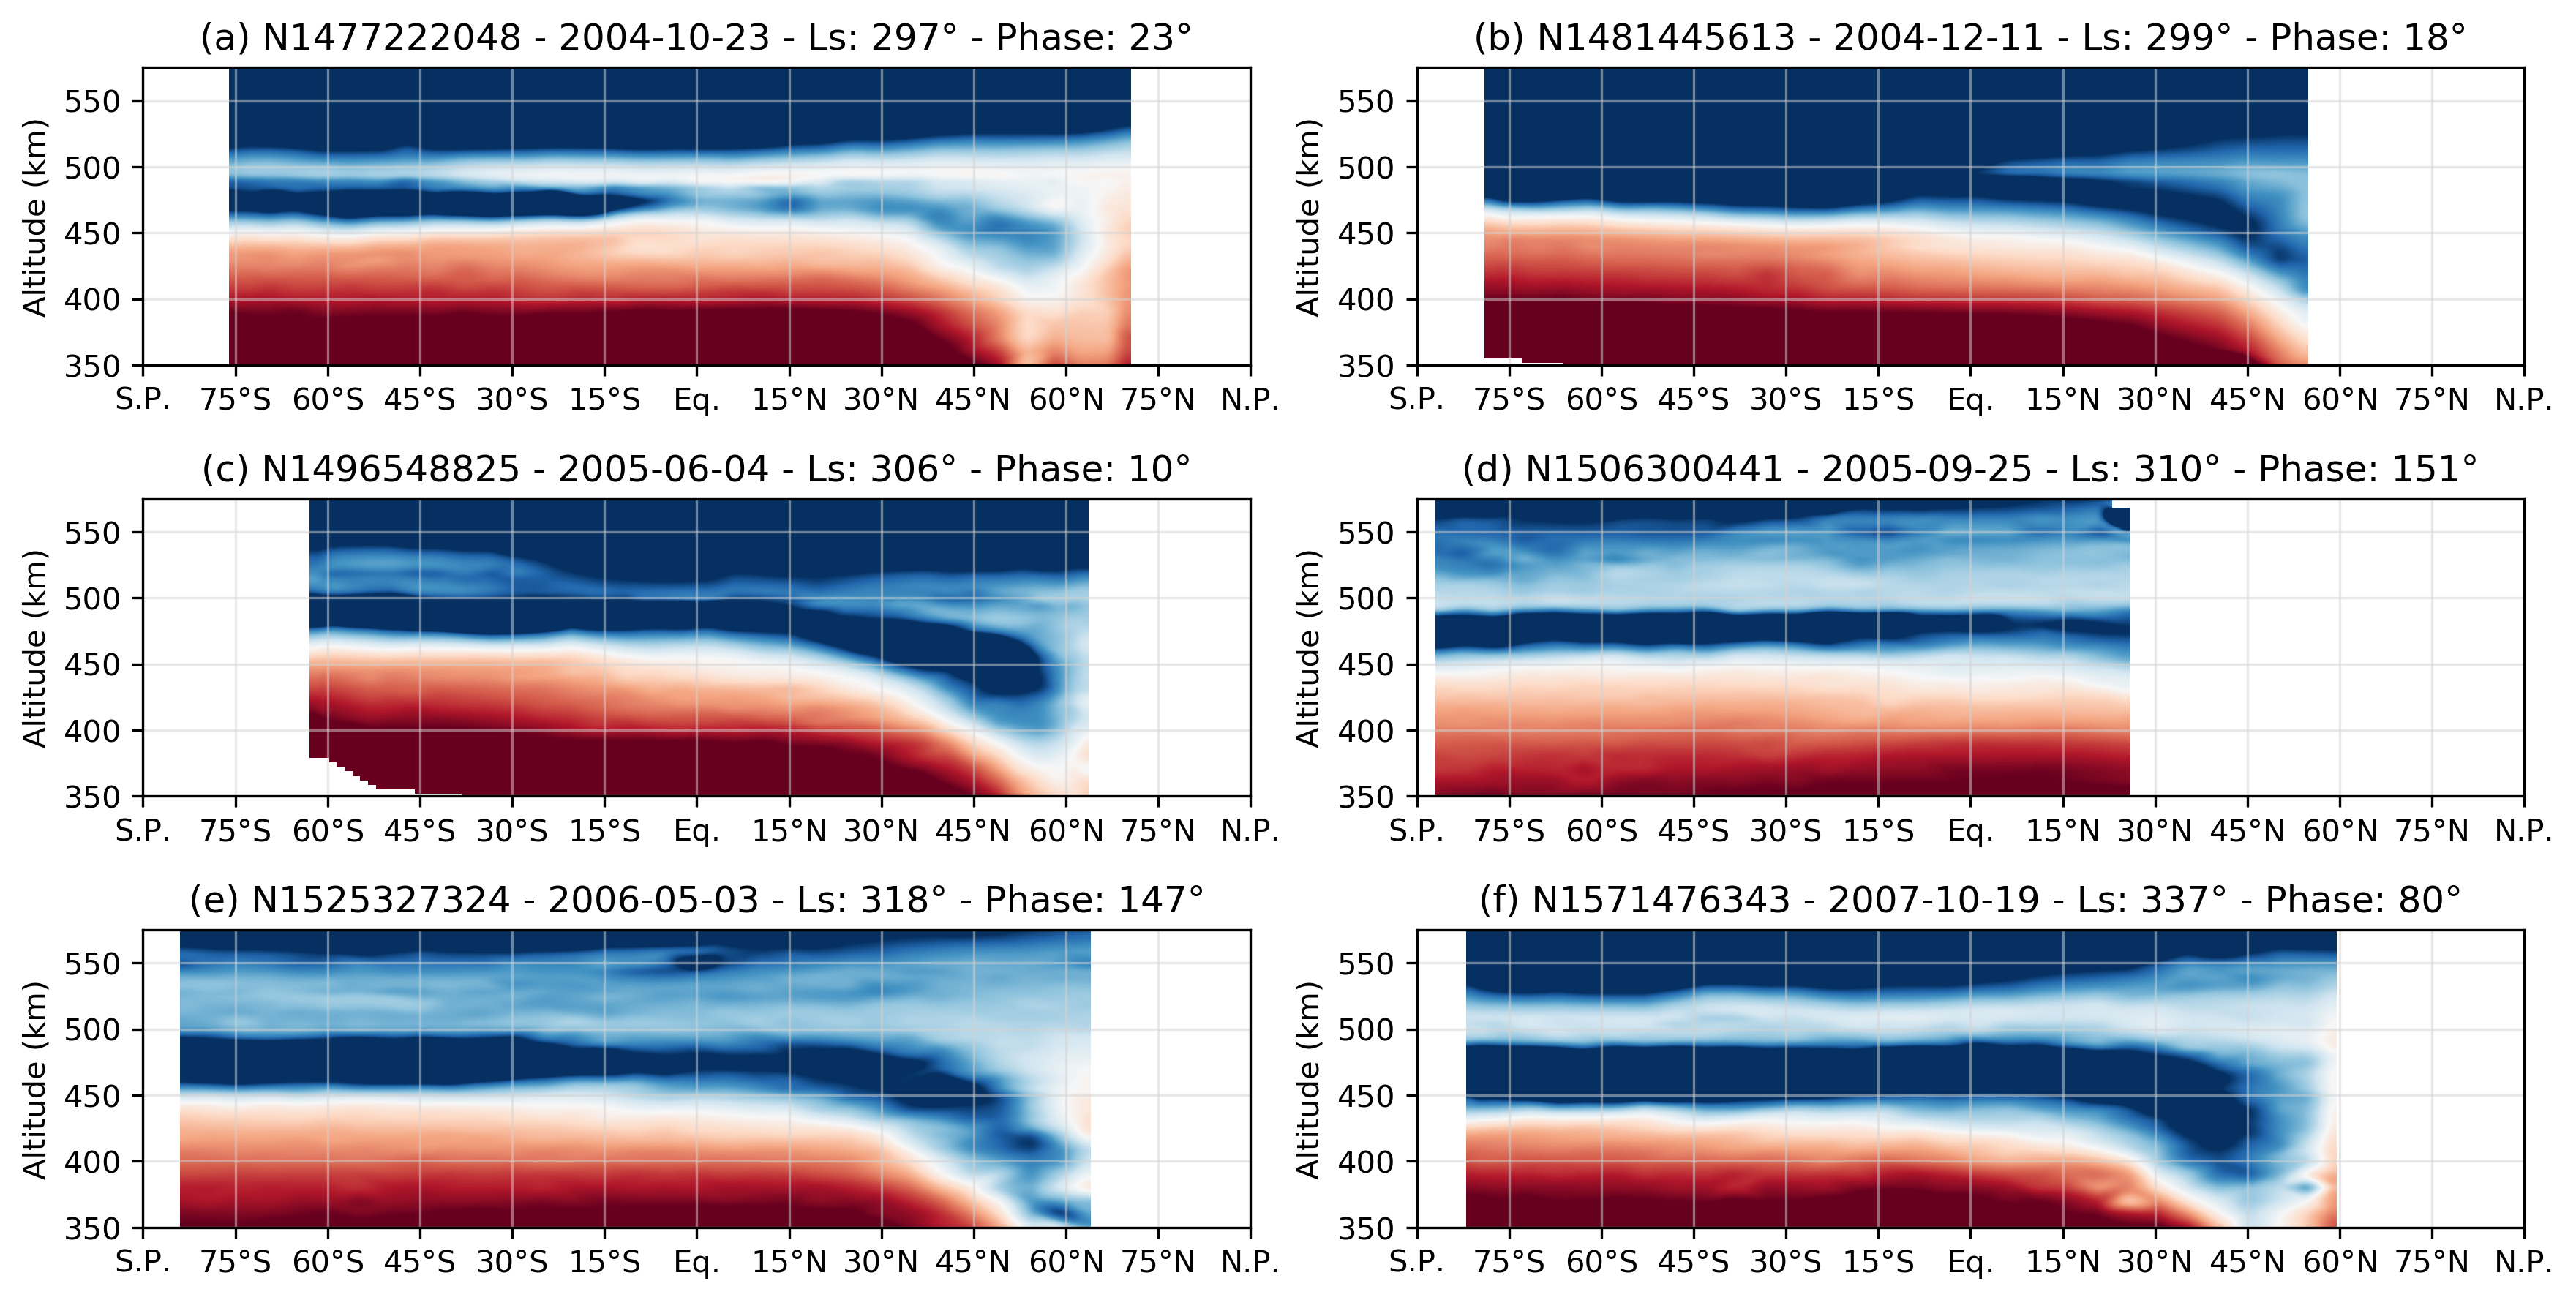
\includegraphics[width=\textwidth]{Fig/Lat_beta-2004_2008.png}
    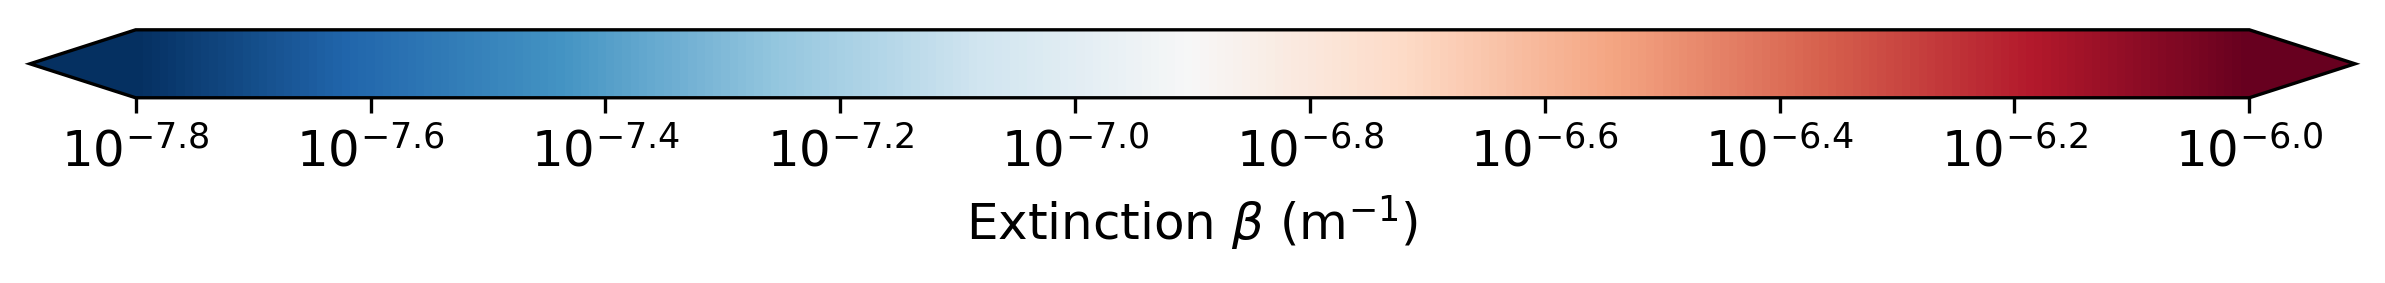
\includegraphics[width=.5\textwidth]{Fig/Extinction_colorbar.png}\vspace{-.3cm}
    \caption{Latitudinal haze extinction profile ($\beta$) retrieved for 6 images taken between 2004 and 2008
    ($L_s=\ang{300}-\ang{340}$) showing a stable DHL at $500 \pm 20$ km altitude.
    The color schema is fixed for all the figures to make direct comparison
    between the different panels. The seasonal solar longitude ($L_s$) and the observation phase angle are
    also provided in each panel.}
    \label{fig:dhl_2004_2008}
\end{figure*}

However, there are noticeable variations in haze extinction. During several months, the
detached haze remained stable, but in December 2004 (Fig.~\ref{fig:dhl_2004_2008}b),
the detached haze layer extinction was found to be a factor of 10 lower than previously at almost all latitudes south
of \ang{30}N, and about half a decade above \ang{30}N. The polar hood and the main haze do not show a similar decrease.
In the following periods, (Fig.~\ref{fig:dhl_2004_2008}c, d and e),
the detached haze was partially restored, but not with the same amount of extinction as before. Only observations in
2007 (Fig.~\ref{fig:dhl_2004_2008}f) show extinctions in the detached haze layer comparable to those seen before
the decrease. We note that the decrease of extinction below 370 km in the polar hood above \ang{50}N
(Fig.~\ref{fig:dhl_2004_2008}e) is at the limit of sensitivity of the UV filter. The stability of the large-scale
structure of the detached haze layer is related to the steady state of the large-scale circulation during all the winter.
The observation of October 2007 (Fig.~\ref{fig:dhl_2004_2008}f) is the last view that we have of this stable state
before the seasonal turnover.

During this period, the detached haze also has a strong layering with, at some latitudes, distinct decks which are not
continuous and rather appear as foliation. This feature is more pronounced in some observations, for instance from
June 2005 to May 2006, but does not shows up in October 2007, except marginally beyond \ang{30}N. The foliated detached
haze layer has a larger geometrical thickness than before December 2004.

% NOTE: [PR] We should really check that the apparent difference in geometric thickness of the DHL is not due to something else, as for instance, the phase angle. It could be due to a real effect of some aerosols above the DHL which scatter in a different way than aerosols in DHL itself. Or it could be due to a deconvolution effect that could differ depending on the appearance of Titan as a full disk or a crescent...

As we will see in the \textbf{section 4}, the detached haze layer exhibits some longitudinal or diurnal variability
that limits our ability to interpret details of features observed in single images. The small-scale features
could depend on the local short-term dynamics such as initia-gravity waves.

\subsection{Period 2: Drop and disappearance of the main haze layer around the Vernal Equinox (2008-2012) - $L_s=\ang{340}-\ang{30}$}

A precursor sign of the drop of the detached haze can be seen in March 2008 (Fig.~\ref{fig:dhl_2008_2012}a).
The main haze starts an initial contraction, perceptible around \ang{35}S. There, the depleted zone is almost
75 km thick at its maximum. In January 2009, the main haze continued to fall down from 425 km down to 375 km
while the detached haze layer remained around 500 km (Fig.~\ref{fig:dhl_2008_2012}b). After the drop
of the main haze in early 2009, the detached haze starts its own descent in June 2009, just before the equinox
(Fig.~\ref{fig:dhl_2008_2012}c). This delay in collapse increased the apparent thickness of the depletion
zone between the two haze layers.

\begin{figure*}[!ht]
    \centering
    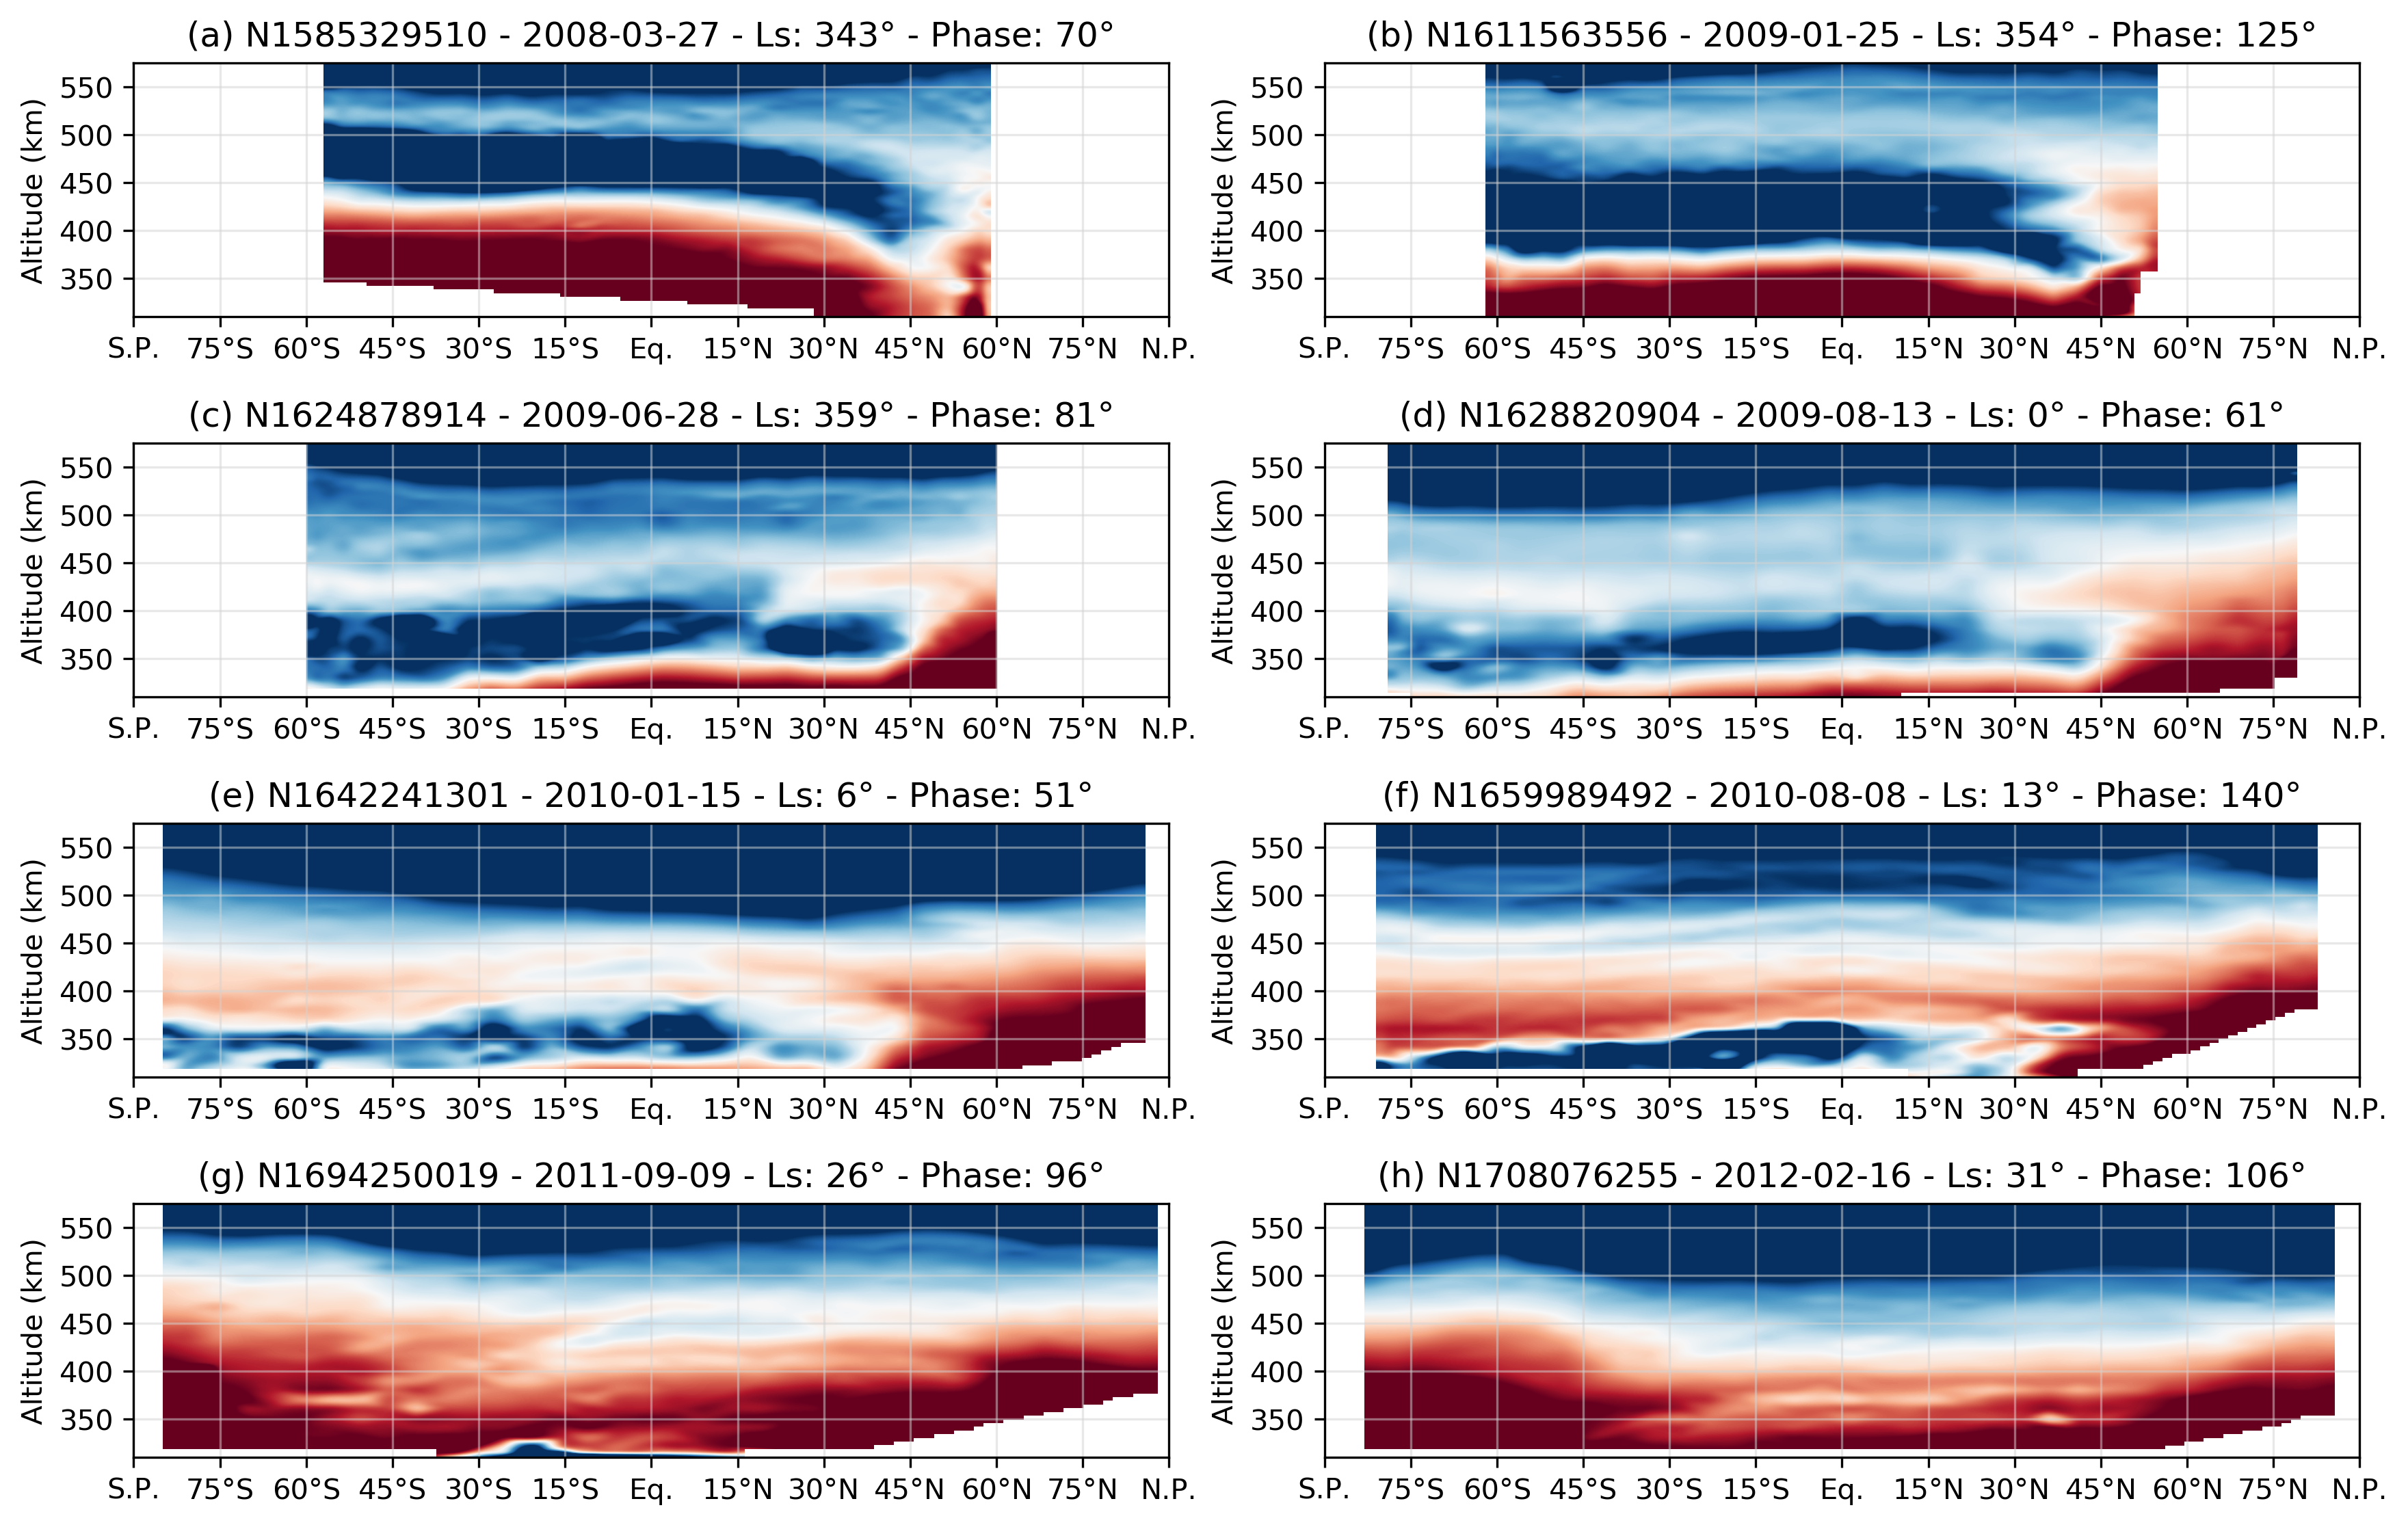
\includegraphics[width=\textwidth]{Fig/Lat_beta-2008_2012.png}
    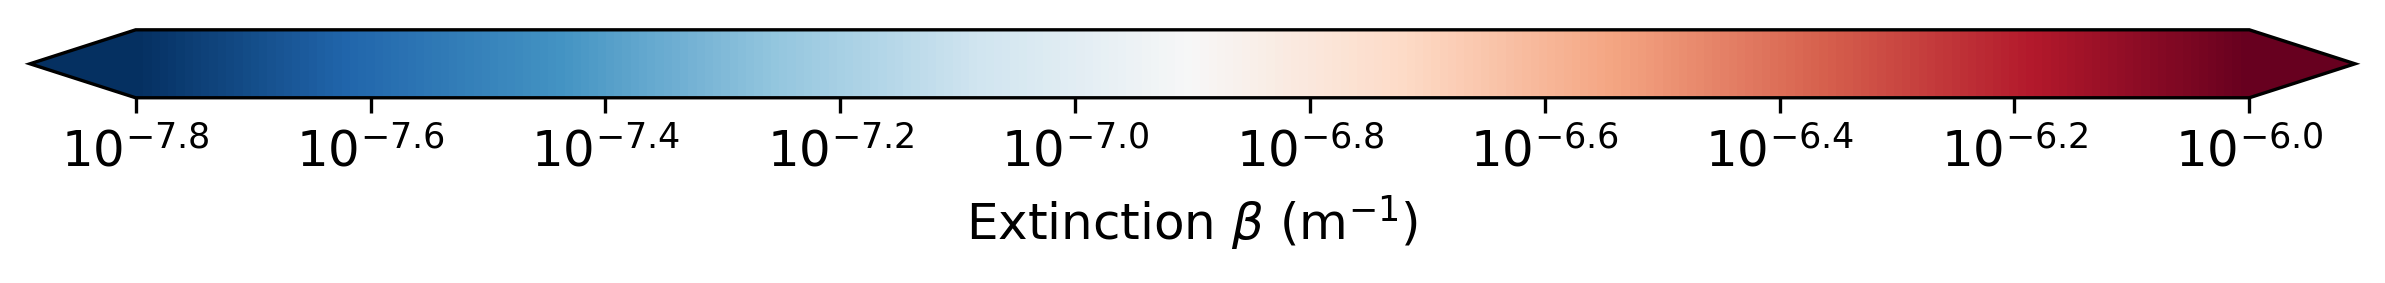
\includegraphics[width=.5\textwidth]{Fig/Extinction_colorbar.png}\vspace{-.3cm}
    \caption{Same as the figure~\ref{fig:dhl_2008_2012} for 8 images taken between 2008 and 2012
    ($L_s=\ang{340}-\ang{30}$) showing the collapse of drop and disappearance of the DHL.
    The color schema extent is kept similar to the figure~\ref{fig:dhl_2008_2012} to provide
    direct comparisons but the altitude range is extended down to 300 km around the UV3 saturation
    level (where the atmosphere is opaque).}
    \label{fig:dhl_2008_2012}
\end{figure*}

As for the main haze, the detached haze collapses first in the South hemisphere, from 500 km to 425 km, and
then at equator and in the northern hemisphere (Fig.~\ref{fig:dhl_2008_2012}c).
This is associated to the circulation turnover affecting first the summer hemisphere ascending branch.
With time, the detached haze gradually settled in altitude and finally merged with
the main haze. The complete collapse of the detached haze is displayed in Fig.~\ref{fig:dhl_2008_2012}c to
Fig.~\ref{fig:dhl_2008_2012}h. We note that the extinction of the detached haze is smaller at equator than at
other latitudes, and this will be the case during all the drop.

During the fall, a second thin detached haze layer, at planetary scale, can be remarked above the collapsing detached
haze layer. In January 2010 (Fig.~\ref{fig:dhl_2008_2012}e), the detached is now located between 375 and 400 km.
We can still see a double deck of haze, and this time the detached haze appears higher at the equator compare to the two
hemispheres, producing an arch. The haze extinction has globally increased by a factor of two due to sedimentation
in denser layers.

In August 2010 (Fig.~\ref{fig:dhl_2008_2012}f), one year after equinox, the detached haze layer continued
its drop down to 350 km around \ang{40}N and 400 km at the equator. It has gained in complexity with
multiple secondary layers up to 520 km. The detached haze form a remarkable arch with a difference of about 50 km
in altitude between the equator and the poles as previously noticed by~\cite{West2011}.
This observation and the next one correspond to the same time of the
year than the time of Voyagers flybys ($L_s=\ang{8}$ and \ang{18}). They can be compared quite directly. We now know
that this season was a time of rapid change, and that the Voyager probes observed transient situations. Voyager also
observed the detached haze higher near equator than elsewhere \citep{Rages1983, Rannou2000}. This corresponds to
the detached haze layer following an isobar level.

Due to orbital constrain and mission planning, the next observation was made in September 2011
(Fig.~\ref{fig:dhl_2008_2012}g). The detached haze layer is now well below the level of the polarhoods.
Again secondary detached layers show up as high as 470 and 520 km.
The south polarhood was not present in January 2010 (Fig.~\ref{fig:dhl_2008_2012}e), it could not be seen
neither northward to \ang{70}S in August 2010 (Fig.~\ref{fig:dhl_2008_2012}f). We conclude that it was surely
built in less than 20 months, and may be less than seven months. The circulation started to reverse around the equinox
and the southward circulation send haze in the south pole and produced this polarhood. The change in haze distribution
is a very good indication of the timing of the equinoctial circulation turnover, has it is discussed later. We note
that the strong haze depletion at 300 km and between \ang{30}S and \ang{20}N is real but may be exaggerated at \ang{20}N
due to the limit of the retrieval procedure. At this altitude level, Titan's atmosphere is opaque to UV radiations
(see Fig.~\ref{fig:model_uncertainties}) and does not allow use to follow the main depletion below this altitude.

The last image that we have with a detached is February 2012 (Fig.~\ref{fig:dhl_2008_2012}h). At that
time, the initial detached haze has completely disappeared and the secondary detached hazes is still descending
and reach 400 km. The secondary detached hazes is not well delineated by a layer strongly depleted in aerosols.
The south polarhood increases its latitudinal extent northward to \ang{50}S and becomes larger than the northern
polarhood which tends to decrease.

\subsection{Period 3: Absence of DHL with sporadic transitory layers after the Northern Spring Equinox (2012-2015) - $L_s=\ang{30}-\ang{75}$}

During this period, the main haze layer has large scale structures which slowly evolve under the influence of the
large scale circulation. The south and north polarhoods are still visible and they evolve
with time. Superimposed to this background haze, transient structures show up and disappear from one observation
to the other. At some moments, large scale detached hazes appear. They differ from the detached haze seen at the
beginning of the mission because they are not stable in time and in altitude. They do not appear from one
observation to the other. The haze during this period is displayed in Fig.~\ref{fig:dhl_2012_2015}.

\begin{figure*}[!ht]
    \centering
    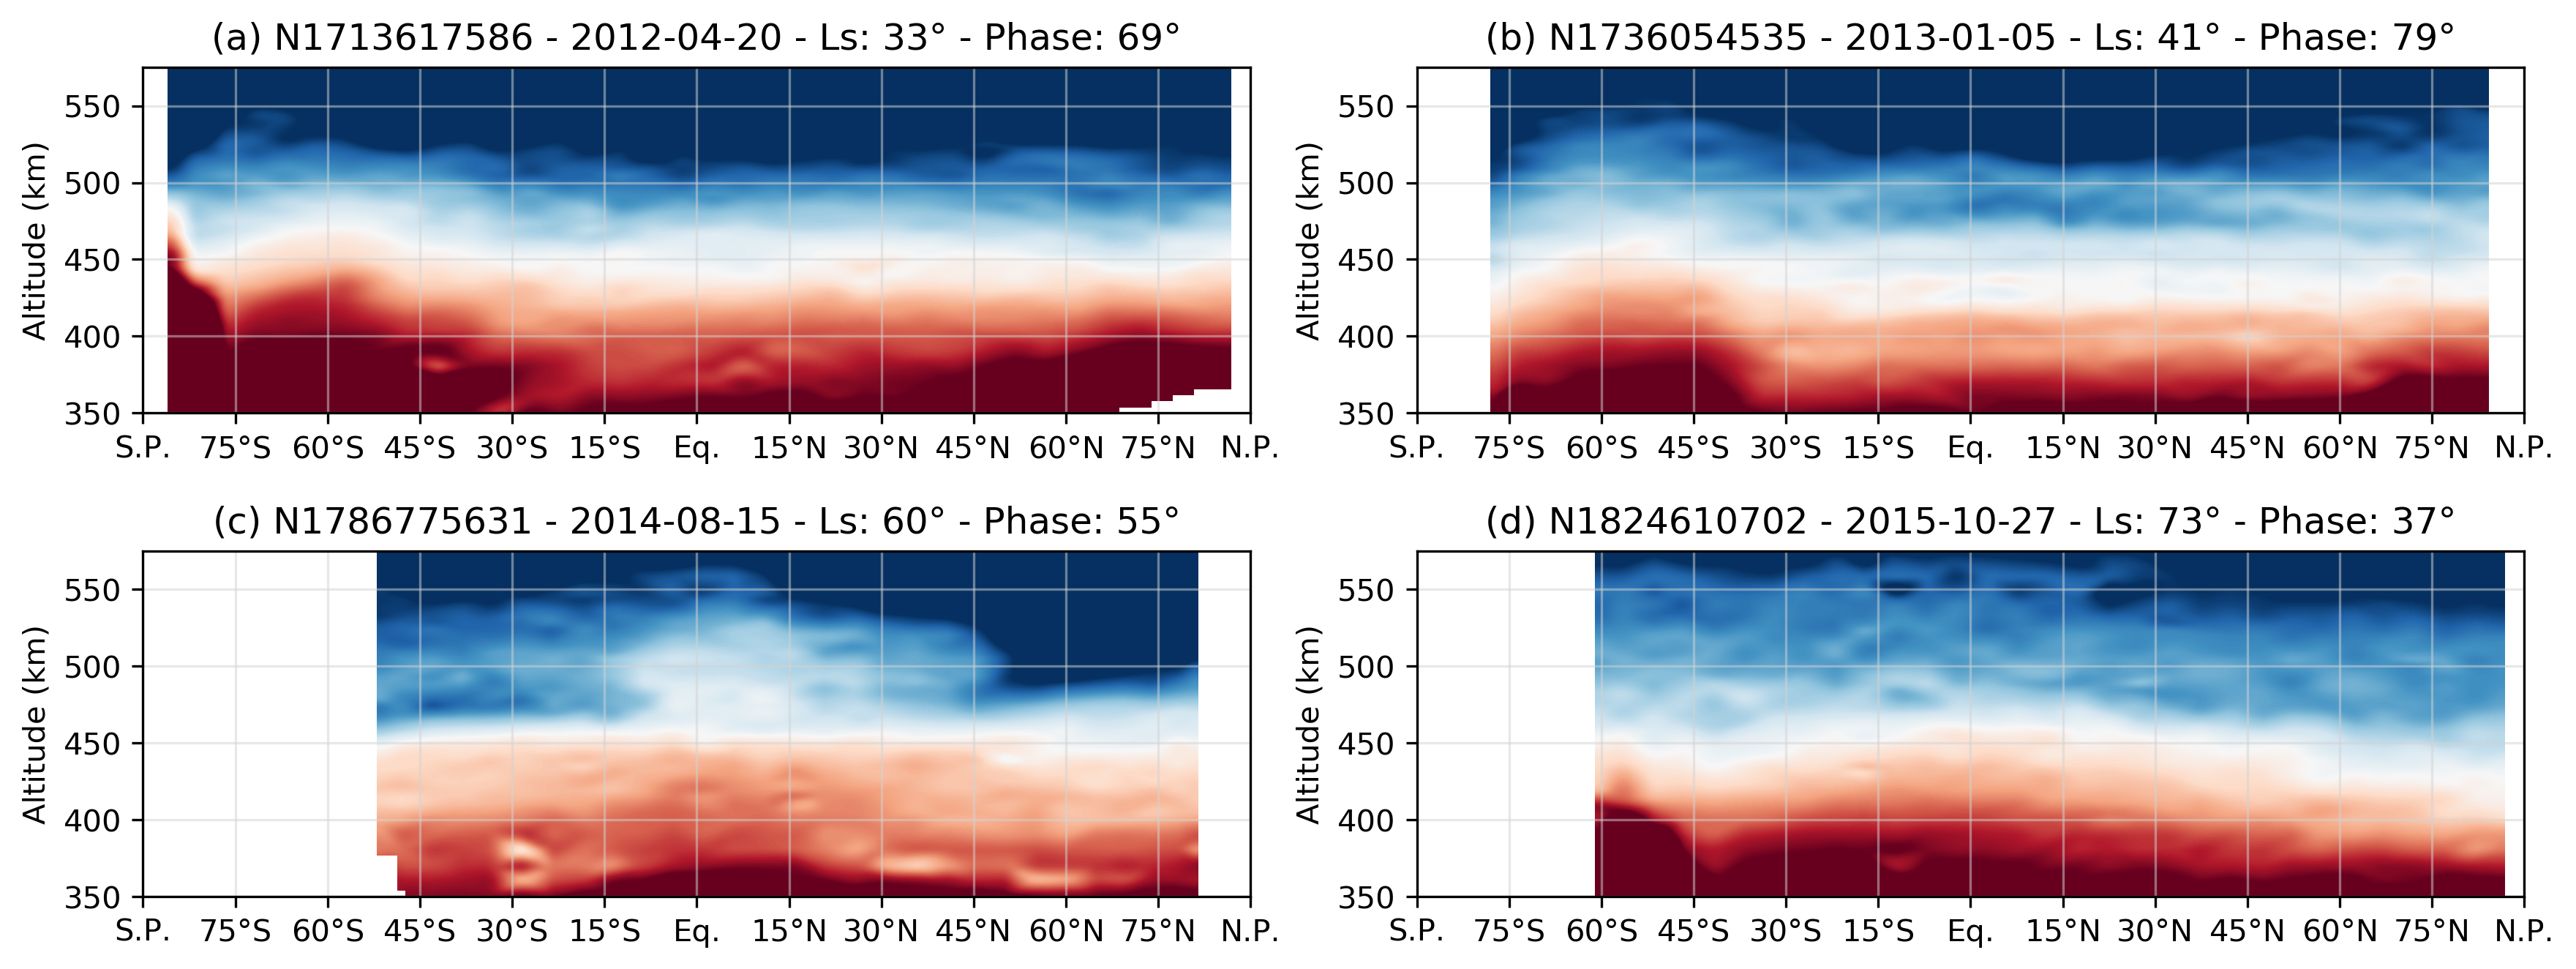
\includegraphics[width=\textwidth]{Fig/Lat_beta-2012_2015.png}
    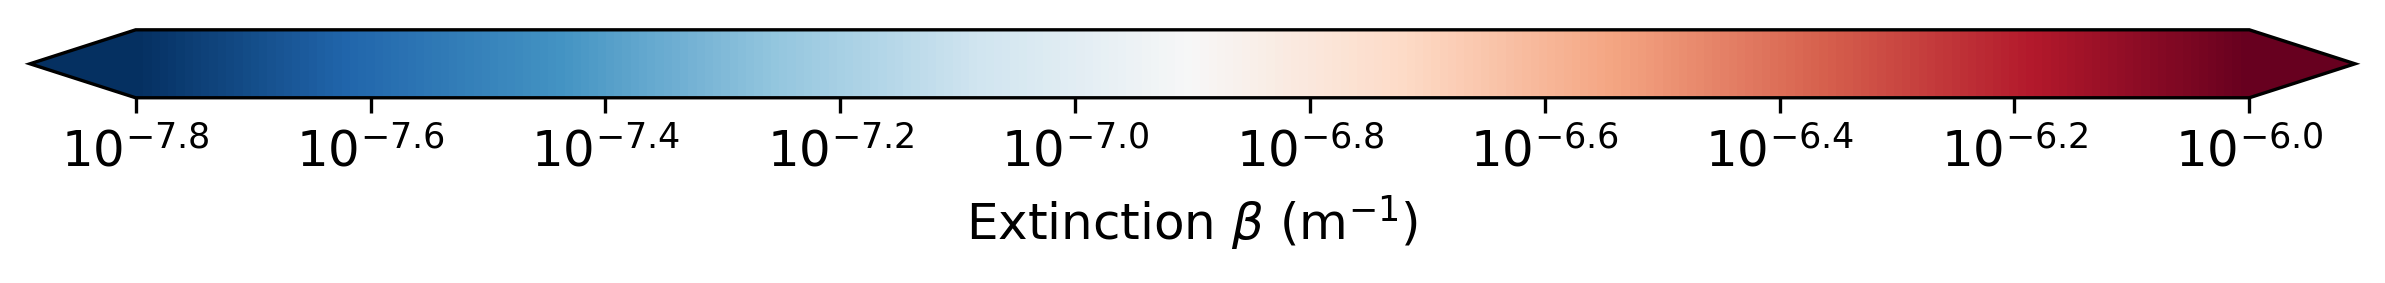
\includegraphics[width=.5\textwidth]{Fig/Extinction_colorbar.png}\vspace{-.3cm}
    \caption{Same as the figures~\ref{fig:dhl_2004_2008} and~\ref{fig:dhl_2008_2012}
    for 4 images taken between 2012 and 2015 ($L_s=\ang{30}-\ang{75}$) showing sporadic
    transitory layers and the absence of consistent DHL.
    The color extent is the same and the altitude ranges down to 350 km.}
    \label{fig:dhl_2012_2015}
\end{figure*}

In April 2012 (Fig.~\ref{fig:dhl_2012_2015}a), the detached haze has completely disappeared, except a residual
structure at \ang{5}-\ang{20}S, around 370 km.
This relict of the last detached haze layer is almost not perceptible in the corresponding I/F profile. At other
latitudes, we only can see a unique main haze with a marked south polarhood and a small increase of extinction above
\ang{65}N that could be the north polarhood. Sometimes, detached layers emerge from the background with large latitudinal
extent (e.g. detached haze at 500 km Fig.~\ref{fig:dhl_2012_2015}b). However, they only remain for a short time
and are not seen in the following observations.

In August 2014 (Fig.~\ref{fig:dhl_2012_2015}c) we observed a plume of aerosol between \ang{10}S and \ang{25}N,
at 500 km. A detached haze layer seems to have spread from this plume toward the north and the south. This
detached haze is around 500 km, descending to 470 km at \ang{60}S (and probably even southern). At the
north, the detached haze does not extend northern than \ang{50}N and remains at 500 km. This indicate an
atmosphere circulation rather flowing from equator toward the south pole. The origin of these aerosols is undefined.

The observation of October 2015 (Fig.~\ref{fig:dhl_2012_2015}d) is very representative of the haze layer in
the period between 2012 and the end of 2015. At this date, the main haze has a uniform scale height of 45 km and
with a homogenous extinction at the planetary scale.

\subsection{Period 4: Reappearance of a new detached haze layer around the Summer Solstice (2015-2017) - $L_s=\ang{75}-\ang{95}$}

The first occurrence of the detached haze in this period is the 3$^{rd}$ December 2015
(Fig.~\ref{fig:dhl_2015_2017}a). Strictly speaking, it
does not differ from the previous sporadic detached haze layers observed in the period 2012-2015. But, after
this observation, the detached haze was present in each observations. The detached haze became stable in time,
similarly to the detached haze before the equinox. Therefore, we consider this date as the beginning of the
reappearance of the detached haze ($L_s=\ang{74}$). The evolution of the haze during this period is displayed in
Fig.~\ref{fig:dhl_2015_2017}. The observations validate the long awaited reappearance of the detached haze layer,
just before the end of the Cassini mission in September 2017.

\begin{figure*}[!ht]
    \centering
    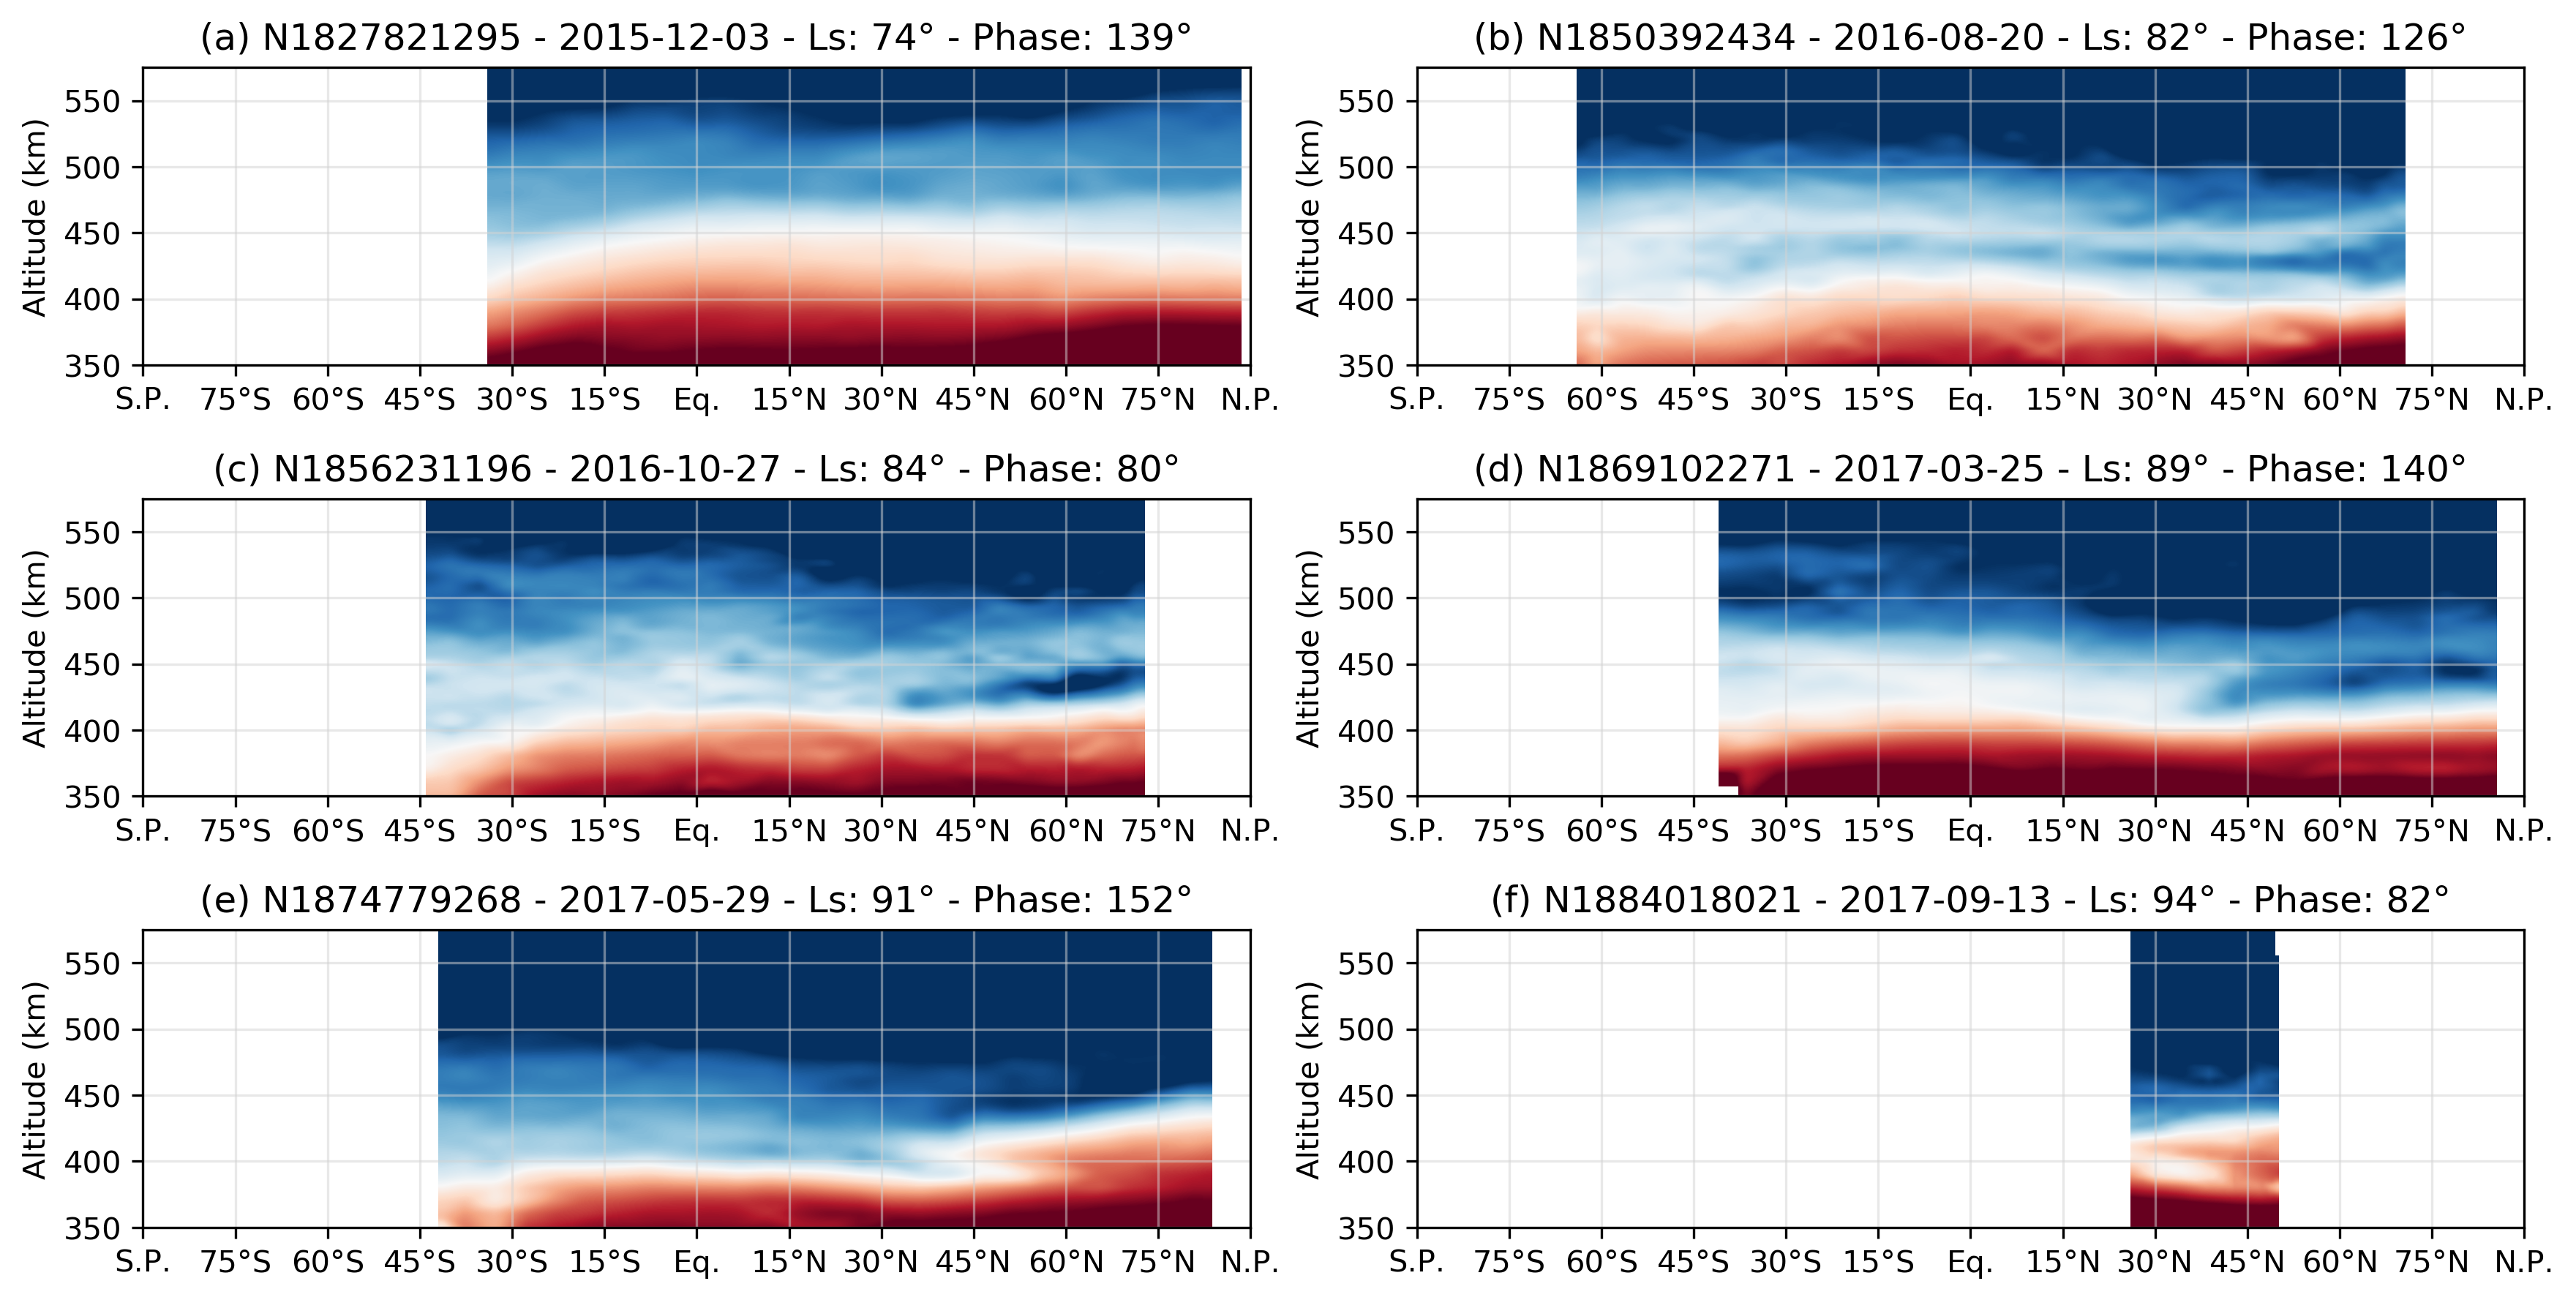
\includegraphics[width=\textwidth]{Fig/Lat_beta-2015_2017.png}
    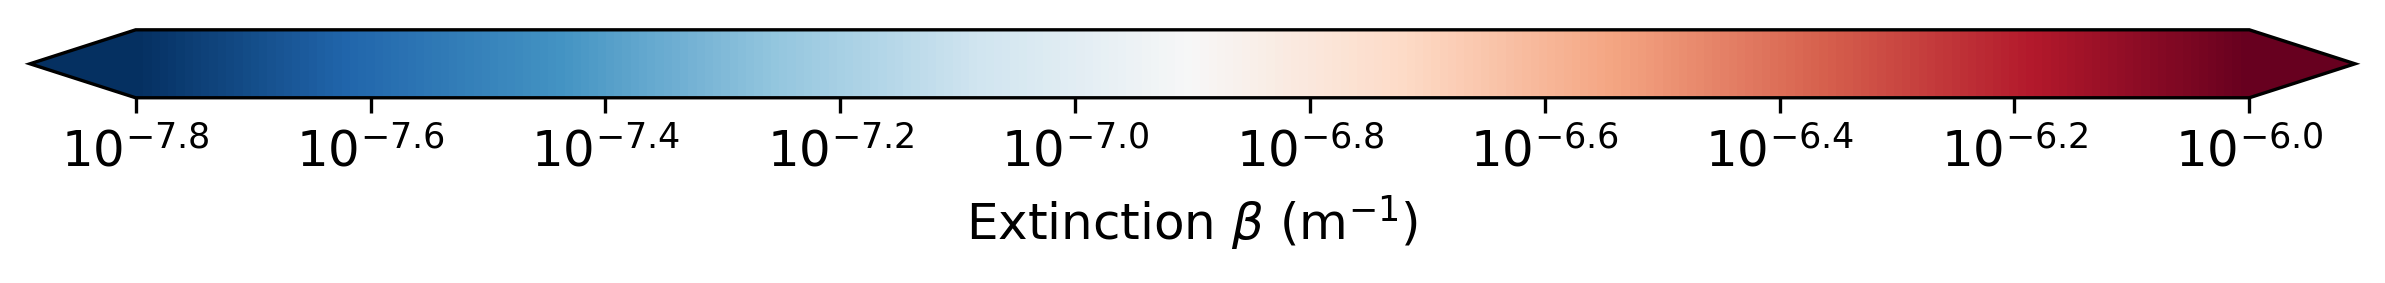
\includegraphics[width=.5\textwidth]{Fig/Extinction_colorbar.png}\vspace{-.3cm}
    \caption{Same as the figures~\ref{fig:dhl_2004_2008}, \ref{fig:dhl_2008_2012}
    and~\ref{fig:dhl_2012_2015} for 6 images taken between 2015 and 2017
    ($L_s=\ang{75}-\ang{95}$) during the reappearance of the DHL.
    The image \textbf{N1884018021\_1} is one of the very last observation of Titan before
    the end of the Cassini mission in September 2017.}
    \label{fig:dhl_2015_2017}
\end{figure*}

At the beginning, the detached haze layer is not very well defined but it can be perceived at all latitudes
around 490 - 520 km (Fig.~\ref{fig:dhl_2015_2017}a). We notice at the same moment a contraction
the main haze, with the top of the haze dropped by 50 km in January 2016 compared to October 2015
(Fig.~\ref{fig:dhl_2012_2015}d). The main elements of the reappearance (altitude and date) confirms the
predictions made by the general circulation models \citep{Lebonnois2012,Larson2015} and the prediction
reported in \cite{West2011}. The detailed comparison between the observations and GCM is discussed further.

With time, the detached haze layer is better marked and the zone of depletion is more pronounced, especially in the
northern hemisphere (Fig.~\ref{fig:dhl_2015_2017}b). The situation seems to be analogue to an early stage of
the structure observed in 2004 (with the opposite latitude). However, although the detached haze persists in time,
it also settles and almost merges with the main haze in October 2016 (Fig.~\ref{fig:dhl_2015_2017}c).
In the  following observations (Fig.~\ref{fig:dhl_2015_2017}d and Fig.~\ref{fig:dhl_2015_2017}e), we are
witnessing the complex evolution of the first appeared detached haze that merge with the main layer at latitude southward
to $\simeq \ang{35}$N while it remains stable around 450 km northward to \ang{35}N and seems to vanish rather than settle.
This structure was still observed in the very last image of Titan taken by Cassini just before its last plunge into Saturn
atmosphere (Fig.~\ref{fig:dhl_2015_2017}f) in September 2017.

A secondary detached haze layer appears in the southern hemisphere at high altitude around 520 km
(Fig.~\ref{fig:dhl_2015_2017}c). Its northern boundary is not well defined. This new structure will be persistent with
time, at planetary scale up to the end of Cassini mission but is gradually descending. The results reported by \cite{West2018}
concerns the detached haze at equator only. Although they already revealed a complex behavior of the detached haze layer, the
present observations show a dichotomy between the two hemispheres. The detail of the evolution, the split in a double layer
structure, the formation and disappearance of several structures was completely unexpected. According to GCMs, six years
after equinox, the post-equinoctial circulation was supposed to be already installed with a planetary scale circulation cell
from the south hemisphere to the north polar region. Apparently, this is not the case.

These observations from 2004 to 2017 does not completely cover half a Titan year. The first and last observations
were taken almost at the opposite season, $L_s=\ang{297}$ and \ang{94} respectively (\emph{i.e.} \ang{157} apart).
This prevents direct comparisons between the detached haze at the beginning and at the end of the mission,
although in both cases they are taken more than a season after the previous solstice.
